\section{Implementation of Boneh-Franklin based IBE and Results }
\label{sec:bfibe.imp}


For elliptic curve point multiplication, there are potentially exploitable side-channel attacks that arise from using the classic \textit{double-and-add} algorithm and its variants. Vulnerabilities arise if branches are taken that depend on secret bits, or if data is even accessed using secret values as indices.\cite{lib.miracl.report} 

As a counter-measure the simplest solution is to use
a constant-time algorithm like the \textit{Montgomery ladder}, which  uses very little memory and has no key-bit-dependent branches. Other suggestions for representation may be the \textit{fixed-sized signed window method}. To tackle down the pairings related hash-to-curve problems and the previously mentioned reasons we choosed to use MIRACL Core library\cite{lib.miracl}. 

MIRACL Core has built-in support for most standardised elliptic curves,
along with many curves that have been proposed for standardisation. As we previously mentioned is \textit{Section \ref{sec:apx.ecc.curves.pairing}} BN and BLS curves are specific elliptic curves whose supporting pairing based cryptography. These are the so-called Type-3 pairings. The MIRACL Core library provides optimized functions for pointt multiplications in the elliptic curve groups $\mathbb{G}_1, \mathbb{G}_2$ and exponentiation in a finite extensions field $\mathbb{G}_T$ and for the pairing itself.\cite{lib.miracl.report}


The \textit{MIRACL-core}\cite{lib.miracl} implementation of Identity-Based Encryption (IBE) utilizes the BLS12-381 pairing-friendly elliptic curve to allow encryption using arbitrary identity strings such as email addresses. The core cryptographic architecture is organized into four classes: \texttt{Setup}, \texttt{Extract}, \texttt{Encrypt}, and \texttt{Decrypt}, along with the supporting \texttt{Ciphertext} class. The \texttt{Setup} class initializes the cryptographic environment by generating the elliptic curve groups $\mathbb{G}_1$, $\mathbb{G}_2$, and the target group $\mathbb{G}_T$, selecting generators $P \in \mathbb{G}_1$ and $Q \in \mathbb{G}_2$, and generating a master secret $s$. From this secret, the corresponding public keys $P\_pub = sP$ and $Q\_pub = sQ$ are derived. Additionally, \texttt{Setup} provides utility functions such as hashing identity strings to curve points, converting pairing results into byte arrays, deriving random exponents, and generating message masks. For instance, the hash-to-curve operation is implemented via \lstinline|hashToG1|\cite{lib.miracl}:

\vspace{6pt}
\begin{lstlisting}[language=Java, caption={Mapping identity string (hash) to $\mathbb{G}_1$ using ECP.java class}]
	ECP Q_ID = hashToG1(identity);
\end{lstlisting}
\vspace{6pt}

which deterministically maps an identity string to a point on the elliptic curve. The \texttt{Extract} class uses this mapping to compute the private key for a given identity by multiplying the hashed identity point by the master secret:

\vspace{6pt}
\begin{lstlisting}[language=Java, caption={Pairing computation using $G1mul()$ method from ECP java class}]
	ECP d_ID = PAIR.G1mul(Q_ID, masterKey.s);
\end{lstlisting}
\vspace{6pt}

The resulting \texttt{PrivateKey} object contains both the identity and its corresponding private key point.

The \texttt{Encrypt} class performs the encryption of messages intended for a specific recipient. For each message, a random byte array $\sigma$ is generated, which is used along with the message to compute a random exponent $r = H_3(\sigma, M)$. This exponent is used to compute $U = r \cdot P$, which forms part of the ciphertext. The pairing mask is then calculated as $g_{ID} = e(Q_{pub}, Q_{ID})^{H(U)}$, and the ciphertext components $V = \sigma \oplus H_2(g_{ID}^r)$ and $W = M \oplus H_4(\sigma)$ are derived. The complete ciphertext is encapsulated in a \texttt{Ciphertext} object:

\vspace{6pt}
\begin{lstlisting}[language=Java, caption={Masking operations within the Ecrypt.java class}]
	Ciphertext C = new Ciphertext();
	C.U = U;
	C.V = V;
	C.W = W;
	C.recipientIdentity = identity;
\end{lstlisting}
\vspace{6pt}

Decryption is handled by the \texttt{Decrypt} class. Given a \texttt{Ciphertext} and a \texttt{PrivateKey}, the pairing between $U$ and the private key is computed, from which $\sigma$ is recovered. The original message is then reconstructed by XORing the recovered $\sigma$ with $W$, and the correctness is verified using the equality $U = H_3(\sigma, M) \cdot P$. This ensures chosen-ciphertext security and detects any tampering with the ciphertext:

\vspace{6pt}
\begin{lstlisting}[language=Java, caption={ Verification of Chosen-ciphertext security during encryption}]
	// Verification during decryption
	BIG r = hashToZq(sigma, M, params.q);
	ECP expected_U = PAIR.G1mul(params.P, r);
	if (!ciphertext.U.equals(expected_U)) return null;
\end{lstlisting}
\vspace{6pt}

A procedure related to encoding is the conversion of an elliptic curve point to a bit string is called serialization. Typically it is used for compactly storing or transmitting points, as its inverse operation, deserialization, converts a bit string to an elliptic curve point. During deserialization the only difference from encoding in that only certain strings (namely, those output by the serialization procedure) can be deserialized. \cite{ecc.hashing} The \texttt{Ciphertext} class supports serialization and deserialization to facilitate secure transmission between parties:

\vspace{6pt}
\begin{lstlisting}[language=Java, caption={serialization and deserialization }]
	byte[] serialized = C.toBytes();
	Ciphertext restored = Ciphertext.fromBytes(serialized, identity);
\end{lstlisting}
\vspace{6pt}

In addition the implementation enforces cross-identity security, as each identity receives a unique private key, ensuring that only the intended recipient can decrypt a message. Randomization is achieved by generating a fresh $\sigma$ for every encryption, so encrypting the same message multiple times produces distinct ciphertexts. Comprehensive testing verifies correctness of encryption and decryption, proper rejection of invalid keys, tamper detection for altered ciphertext components, and the uniqueness of ciphertexts for repeated encryptions. Lastly the \textit{Picture \ref{fig:bfibetest}} showcases the output of the successful functionality test. For the full result log please refer to \textit{Appedix Section \ref{label}}


\begin{figure}[h!]
	\centering
	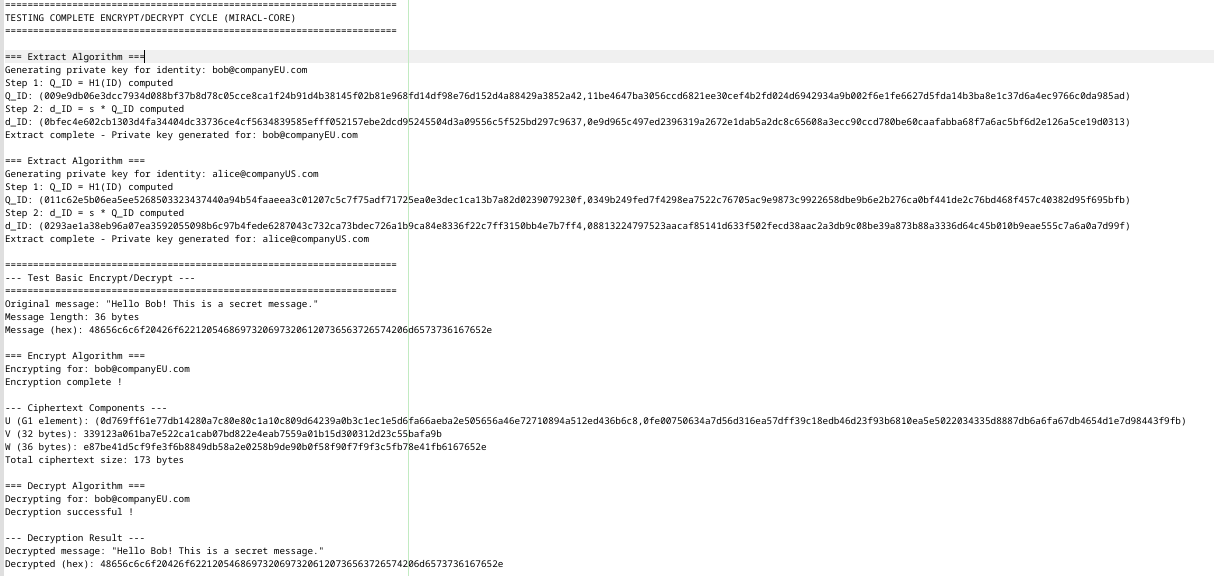
\includegraphics[width=1.0\linewidth]{images/ibetest.png}
	\caption{\textit{BF-IBE scheme functionality test results}}
	\label{fig:bfibetest}
\end{figure}
